\documentclass{article}
\usepackage[letterpaper]{geometry}
\geometry{verbose,tmargin=1in,bmargin=1in,lmargin=1in,rmargin=1in}

\usepackage[utf8]{inputenc}
\usepackage{amsmath}
\usepackage{listings}
\usepackage{graphicx}
\usepackage{enumitem}
\usepackage{amssymb}
\usepackage{tabularx}
\usepackage{hyperref}
\usepackage{caption}
\usepackage{float}
\usepackage[section]{placeins}
\usepackage{empheq}
\usepackage{stackengine}
\usepackage{subcaption}
\usepackage{array}
\usepackage[super]{nth}

\def\delequal{\mathrel{\ensurestackMath{\stackon[1pt]{=}{\scriptstyle\Delta}}}}


\title{CIS 680: Project 2}
\author{Junfan Pan}
\date{10/04/2020}
\begin{document}
\maketitle
    \setcounter{section}{6}
    \section{Submission and Evaluation}
    \begin{enumerate}
    \item[7.5] plot of the mean Average Precision over training\\
    	\begin{figure}[H]
     	\centering
     	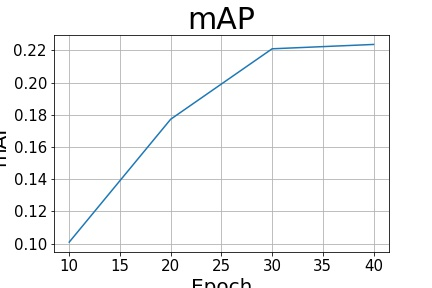
\includegraphics[width=0.7\textwidth]
     	{images/entire_mAP.jpg}
     	\caption{mAP plot}
     	\label{fig:Raw Label}
     	\end{figure}
     	\\
    I plot the mAP for the first 40 training epochs since I observed that after 40 epochs, the mAP constantly decreases.
    \newpage
    \item[7.6 and 7.7] Data Postprocessing
        \begin{figure}[H]
     	\centering
     	\begin{subfigure}[b]{0.45\textwidth}
         	\centering
         	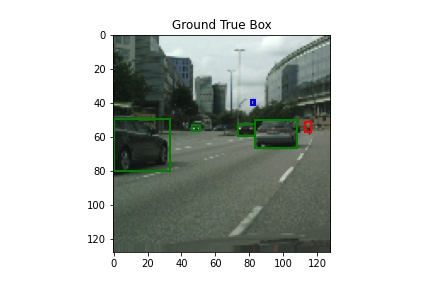
\includegraphics[width=\textwidth]
         	{images/Ground True Box.jpg}
         	\caption{Ground True Box}
         	\label{fig:Hyperplane Epoch 0}
     	\end{subfigure}
     	\hfill
     	\begin{subfigure}[b]{0.45\textwidth}
         	\centering
         	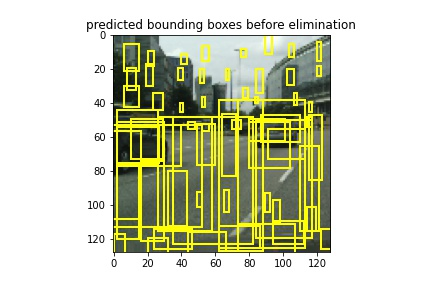
\includegraphics[width=\textwidth]
         	{images/predicted bounding boxes before elimination.jpg}
         	\caption{predicted bounding boxes before elimination}
         	\label{fig:Hyperplane Epoch 1000}
     	\end{subfigure}
     	\end{figure}
     	
     \begin{figure}[H]
        
     	\centering
     	\begin{subfigure}[b]{0.45\textwidth}
         	\centering
         	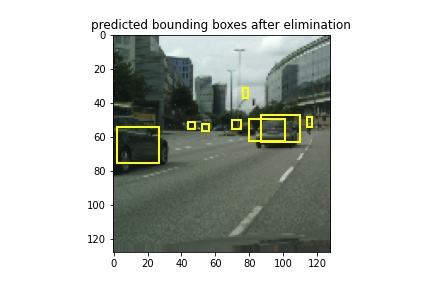
\includegraphics[width=\textwidth]
         	{images/predicted bounding boxes after elimination.jpg}
         	\caption{predicted bounding boxes after elimination}
         	\label{fig:Hyperplane Epoch 0}
     	\end{subfigure}
     	\hfill
     	\begin{subfigure}[b]{0.45\textwidth}
         	\centering
         	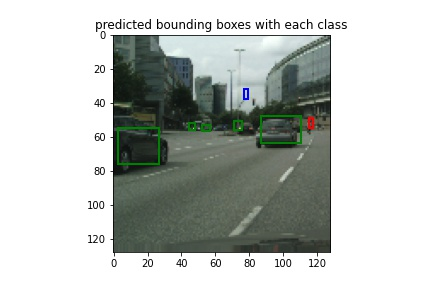
\includegraphics[width=\textwidth]
         	{images/predicted bounding boxes with each class.jpg}
         	\caption{predicted bounding boxes (after NMS) with each class}
         	\label{fig:Hyperplane Epoch 1000}
     	\end{subfigure}
     	\end{figure}

     	\begin{figure}[H]
        \centering
        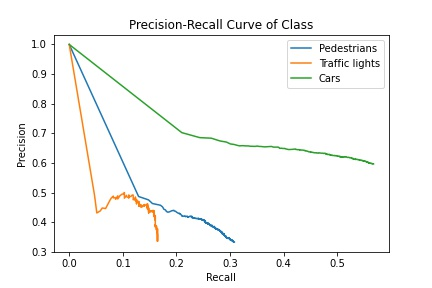
\includegraphics[width=0.6\textwidth]
        {images/Precision-Recall Curve of Class.jpg}
        \caption{precision/recall curves}
        \label{fig:Label}
     	\end{figure}
\\The achieved mean Average Precision for my inference stage is: 0.2237523328559753
\\
     \item[7.8] Issues or challenges
     \item[a.]One issue I encountered is the mismatch between the decrease of the test loss and the worse behavior of object detection. This initially doesn't make sense to me since the reduction of test loss should bring along good performance. However, after I separately plot the test loss of confidence part, classification part and the localization part, I found that the learning speed of these different loss parts are different. Although the total test loss may still decrease, the classification and confidence part have already been overfitted while the localization part is still learning. Therefore, in order to get a better detection performance of small objects such as traffic lights, I should select to use the model checkpoint when the confidence score loss is well-trained and is not overfitted.
     \item[b.]While training my network, I observed that my network can only detect very sparse objects and usually ignore those tiny objects like traffic lights in the figures. Therefore, to eliminate the impact of the small size on detection performance, I set the C$_$target as 1 instead of using confidence score from iou. This enabled my network to detect more small objects and from the figures from the 7.7, the network can now succeed in detecting small objects.
     \item[c.]If more time allowed, I would definitely spend more time on training a more well-behaved network. For example, use more training epochs and introduce a different learning rates during the training process. In addition, instead of setting C$_$target as 1, I can manage to find an appropriate coefficient of the confidence loss part. 
	\begin{figure}[H]
        \centering
        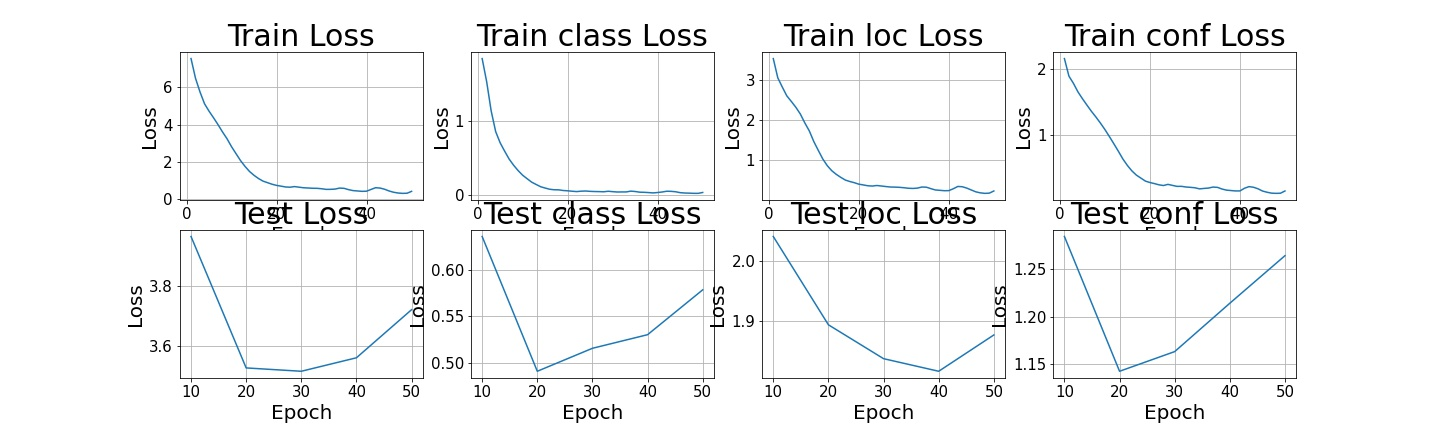
\includegraphics[width=1.1\textwidth]
        {images/test_conf_loss.jpg}
        \caption{different loss parts have different learning rates }
        \label{fig:Label}
     	\end{figure}
    \end{enumerate}
    
        
\end{document}  


